\section{Python应用}

本章的一个重点是能够借助Python,在频域角度分析系统对某输入的作用和输出结果。

本节要点:
\begin{itemize}
    \item 掌握Python分析方法。
\end{itemize}

%============================================================
\subsection{分析方法}

通常有一类问题是已知一个系统,要分析它的对信号产生的作用。
借助Python,一般步骤如下:
\begin{enumerate}
    \item 推导系统频域响应$H\left( \omega \right) $;
    \item 求解信号的傅里叶变换$X\left( \omega \right) $;
    \item 推导输出的时域函数$y\left( t \right) =\mathscr{F} ^{-1}\left[ H\left( \omega \right) \cdot X\left( \omega \right) \right] $。
\end{enumerate}

%============================================================
\subsection{例——RC电路分析}

\begin{example}
如下RC电路,设电压源为输入,电容两端电压为输出,分析不同的RC值对输出的影响。
\begin{figure}[h]
\centering
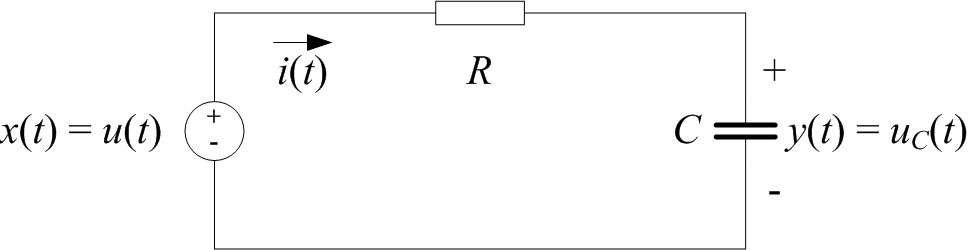
\includegraphics[height=2cm]{1.5.1-1.png}
\end{figure}
\[
x\left( t \right) =p_{\tau =1}\left( t \right) =\begin{cases}
	1,t\in \left[ -0.5,0.5 \right]\\
	0,t\notin \left[ -0.5,0.5 \right]\\
\end{cases}
\]
\end{example}

首先推导系统的频率响应,过程略:
\[
H\left( \omega \right) =\frac{1}{1+i\omega RC}
\]
分别取$RC=1,RC=0.1,RC=0.001$,系统频率响应的频谱图如下。
可见,减小电阻或电容都可以提高系统对高频的响应,特别在$RC=0.001$时,幅频图上看输出几乎没有衰减,相频图上看输出几乎没有相移。

\begin{python}
w  = np.arange(-50, 50, 0.01)
RC = 1;     H1 = 1 / (1 + RC * w * 1.0j)
RC = 0.1;   H2 = 1 / (1 + RC * w * 1.0j)
RC = 0.001; H3 = 1 / (1 + RC * w * 1.0j)

plot_mag_phs(w, np.abs(H1), np.angle(H1, deg=True),
             axs[0][0], axs[1][0], title=r"$H(\omega) ,RC=1$",     ...)
plot_mag_phs(w, np.abs(H2), np.angle(H2, deg=True),
             axs[0][1], axs[1][1], title=r"$H(\omega) ,RC=0.1$",   ...)
plot_mag_phs(w, np.abs(H3), np.angle(H3, deg=True),
             axs[0][2], axs[1][2], title=r"$H(\omega) ,RC=0.001$", ...)
\end{python}

\begin{figure}[h]
\centering
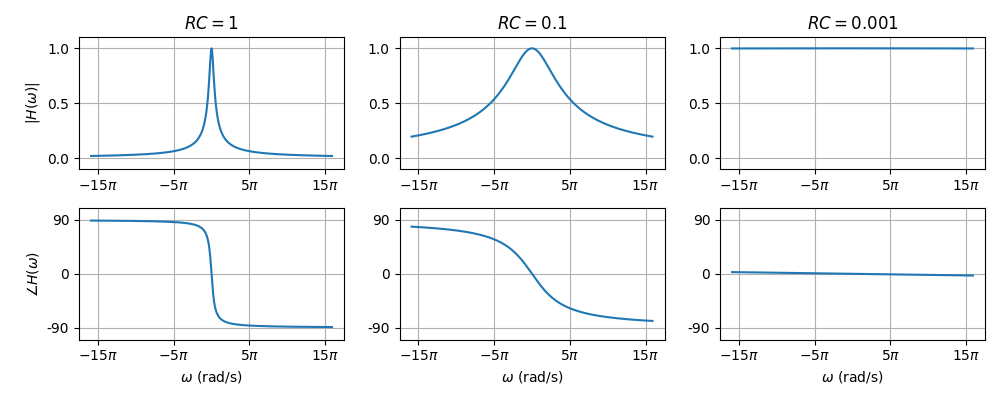
\includegraphics[height=4cm]{5.4.2-1.png}
\end{figure}

再分析输出信号的傅里叶变换,根据单方波的傅里叶变换计算输出的傅里叶:
\begin{align*}
&\because x\left( t \right) =p_{\tau =1}\left( t \right) \leftrightarrow X\left( \omega \right) =\frac{\sin \frac{\omega}{2}}{\frac{\omega}{2}} \\
&\therefore Y\left( \omega \right) =H\left( \omega \right) \cdot X\left( \omega \right) =\frac{1}{1+i\omega RC}\cdot \frac{\sin \frac{\omega}{2}}{\frac{\omega}{2}}
\end{align*}
取$RC=0.5,RC=0.001$,输入和输出的频谱图如下,$RC:0.5\rightarrow 0.001$提高了对输入信号高频部分的响应,使得输出更像输入。
\begin{figure}[h]
\centering
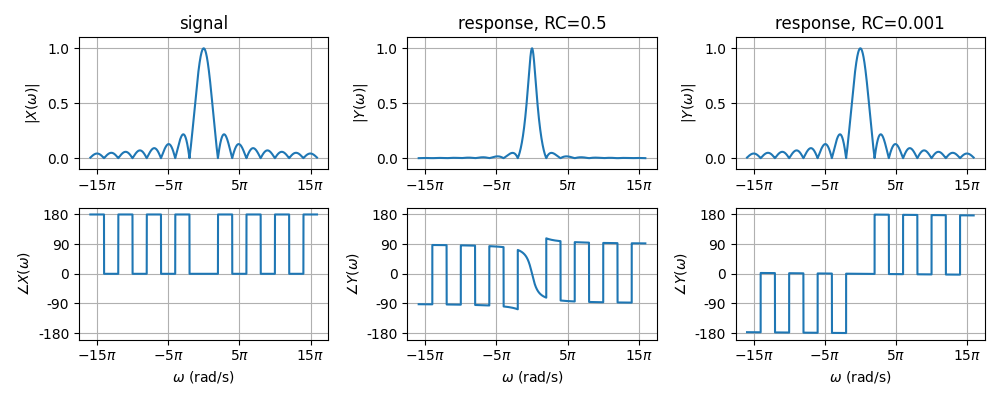
\includegraphics[height=4cm]{5.4.2-2.png}
\end{figure}

\begin{python}
w  = np.arange(-50, 50, 0.01)
X  = (np.sin(w/2) / (w/2))
RC = 0.5;   Y1 = 1 / (1 + RC * w * 1.0j) * (np.sin(w/2) / (w/2))
RC = 0.001; Y2 = 1 / (1 + RC * w * 1.0j) * (np.sin(w/2) / (w/2))

plot_mag_phs(w, np.abs(X),  np.angle(X, deg=True),
             axs[0][0], axs[1][0], title=r"$X(\omega)$",           ...)
plot_mag_phs(w, np.abs(Y1), np.angle(Y1, deg=True),
             axs[0][1], axs[1][1], title=r"$Y(\omega) ,RC=0.5$",   ...)
plot_mag_phs(w, np.abs(Y2), np.angle(Y2, deg=True),
             axs[0][2], axs[1][2], title=r"$Y(\omega) ,RC=0.001$", ...)
\end{python}




